\documentclass[]{report}
\usepackage{graphicx}
\graphicspath{ {resources/images/} }


% Title Page
\title{Utilising peer to peer networking for data transfer over the browser}
\author{Dominic Rathbone}


\begin{document}
\maketitle
\tableofcontents
\


\chapter*{Interim Report}
	\section{Project Scope}
		\subsection*{Aims and Objectives}
			The ultimate objective of my project is to investigate the possibility of data transfer over web browsers (in particular audio and video streaming) without the need for a centralised client-server architecture, instead opting for a peer to peer architecture. In order to do so, I will need to research peer to peer networking as well technologies that will allow for the development of this in the browser such as WebRTC. In order to test and demonstrate this objective, It will materialize in the form of a web application that people can use to both transfer and stream files (if in a suitable format).
		\subsection*{Stakeholders}
			The stakeholders involved in my project will be myself and the supervisor of my project, Stelios Kapetanakis.
		\subsection*{Methods of Communication}
			Stelios and I have set up a regular meeting once a week on friday at 4pm to review progress and answer any questions. On top of this, we communicate regularly via email and I have set up a private git repository on github to keep my project in which I will give Stelios access to.
		\subsection*{Quality Analysis}
		
	\section{Specification}
			The first intermediate deliverable will be a signalling server that will allow my web application to discover two clients and establish the connection between them.
	
	\section{Methodology}
		As a way of tracking the progression of my project, I plan to use the Kanban methodology. Kanban is used within software development as a method of rapid development without overloading developers by restricting them to time-boxed sprints. This methodology is relatively simple and based around a backlog of tasks which developers pull from in a limited amount, normally 1 or 2 tasks at a time which will are then pushed through the development work flow. In my case, the work flow will be relatively simple:
			\begin{enumerate}
				\item Development iteration per task
				\begin{itemize}
					\item Coding
					\item Code Review: Code will be reviewed by self-evaluation, static code analysis and reviews from other students and StackExchange.
					\item Manual Testing: If applicable, black box testing will be used to evaluate the code from a user's perspective.
				\end{itemize}
				\item Stakeholder Approval/User Acceptance Testing: Once all the tasks producing a complete working feature has been produced, it will be tested. 
			\end{enumerate}
		During the coding part of the work flow, I will use a test driven development (TDD) process where I will write the tests first and then write the code to make the test work. However, I will be fairly lenient with this, only using this process on parts of the code that require stringent testing as writing unnecessary tests will take up development time. 
		\begin{center}
			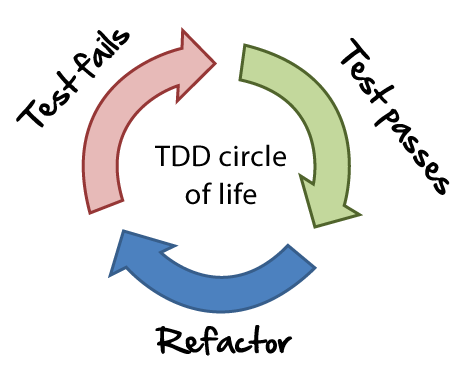
\includegraphics[scale=0.5]{tdd-circle-of-life.png}
		\end{center}
	

	\section{Literature Review}
		\subsection*{Peer to peer networking}
		The entire idea behind my application is based on a one-to-one peer to peer connection between two browsers. Whilst the connection is formed by WebRTC, it does only this, leaving the application to deal with connecting multiple peers together in a “many-to-many” structure resembling a peer to peer network.
		A peer to peer network 


\end{document}          
